\subsection{What is Function-Fiasco}
\begin{frame}
  \frametitle{What is Function-Fiasco}
    \begin{center}
      \huge{\textbf{A Pseudo-tested method detection tool}}

      
\includegraphics[scale = .15]{images/wrench}
    \end{center}
\end{frame}

\begin{frame}[fragile]
  \frametitle{Decorator Function}
  \begin{figure}[t!, scale = .75]
	\begin{lstlisting}[language = Python, basicstyle=\tiny, backgroundcolor = \color{lightgray}]
  def skipper(func):
      functionsComplete = globs.functionsComplete
      checked = checkFunctionsComplete(func, functionsComplete)
      globs.checked = str(checked)
      if checked == True and globs.firstExe == True:
          def wrapper(*args, **kwargs):
              checkType(var, func.__name__)
              return var
          return wrapper
      elif checked == True and globs.firstExe == False:
          def doFunc(*args, **kwargs):
              var = func(*args, **kwargs)
              return checkType(var, func.__name__)
          return doFunc
      else:
          def doFunc(*args, **kwargs):
              var = func(*args, **kwargs)
              return var
          return doFunc
  \end{lstlisting}
\end{figure}
\end{frame}

\begin{frame}
  \frametitle{Execution Flow}
  \begin{center}
    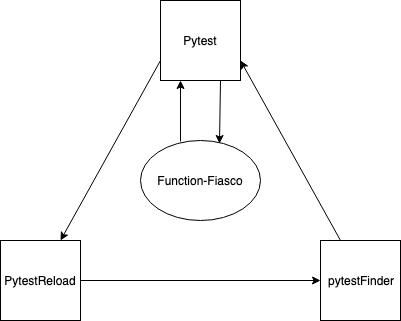
\includegraphics[scale = .5]{images/pytestFlow.png}
  \end{center}
\end{frame}

\subsection{Flow}
\begin{frame}
  \frametitle{Flow to system}
    \begin{center}
      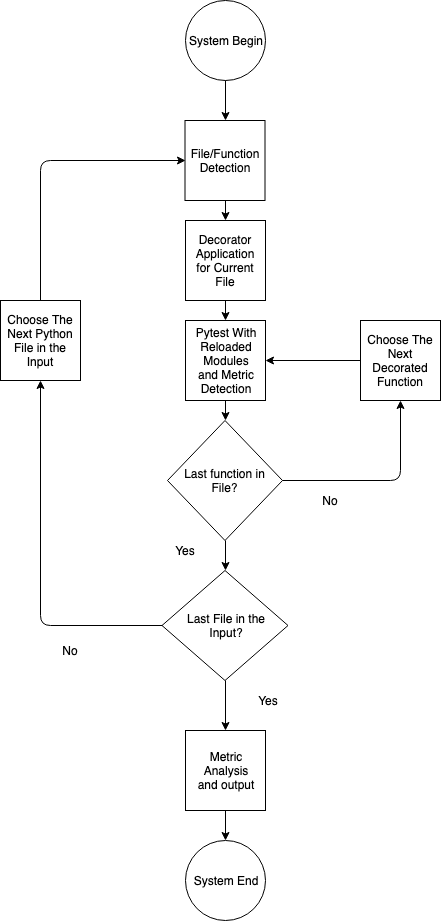
\includegraphics[scale = .22]{images/flow.png}
    \end{center}
\end{frame}
